
\documentclass[11pt]{article}
\usepackage{amsmath,amssymb,amsthm,graphicx,geometry}
\geometry{margin=1in}
\title{NB/BD Stability via a Weighted Hilbert Lemma (v3.2)\\
\large A Classical Analytic Approach toward the Riemann Hypothesis}
\author{Serabi}
\date{\today}

\begin{document}
\maketitle

\begin{abstract}
This work presents version 3.2 of the weighted Hilbert framework for Narrow-Band / Broad-Daylight (NB/BD) stability,
restructured into a rigorously classical analytic number theory (math.NT) direction.
We emphasize Möbius oscillation control, explicit $\eta$-calibration ($\eta \approx 0.35$ with Polya–Vinogradov constant $c_0 \approx 0.7$),
and a zero-free weighted simulation refined by the functional equation symmetry of $\zeta(s)$.
\end{abstract}

\section{Introduction}
We adopt a weighted NB/BD decomposition:
\[
K_{mn} = e^{-\frac{1}{2}|\log(m/n)|},
\]
detecting nontrivial zero structure via Möbius oscillations and mean-square error decay.

\section{Weighted Hilbert Lemma (Revised)}
Let $H_\eta$ act on Möbius-weighted sequences:
\[
(H_\eta f)(m) = \sum_{n \ge 1} e^{-\eta|\log(m/n)|} f(n).
\]
Stability under $\Re(s) > \tfrac{1}{2} + \varepsilon$ yields numerical coherence when $\eta$ is boosted.

\section{Numerical Scaling}
Regression $\log(MSE^*) = a + b\log\log N$ gives:
\[
a \approx -2.915, \; b \approx 0.504 \; (\text{base}); \quad a \approx -0.870, \; b \approx -0.320 \; (\text{boosted}).
\]

\begin{figure}[h!]
\centering
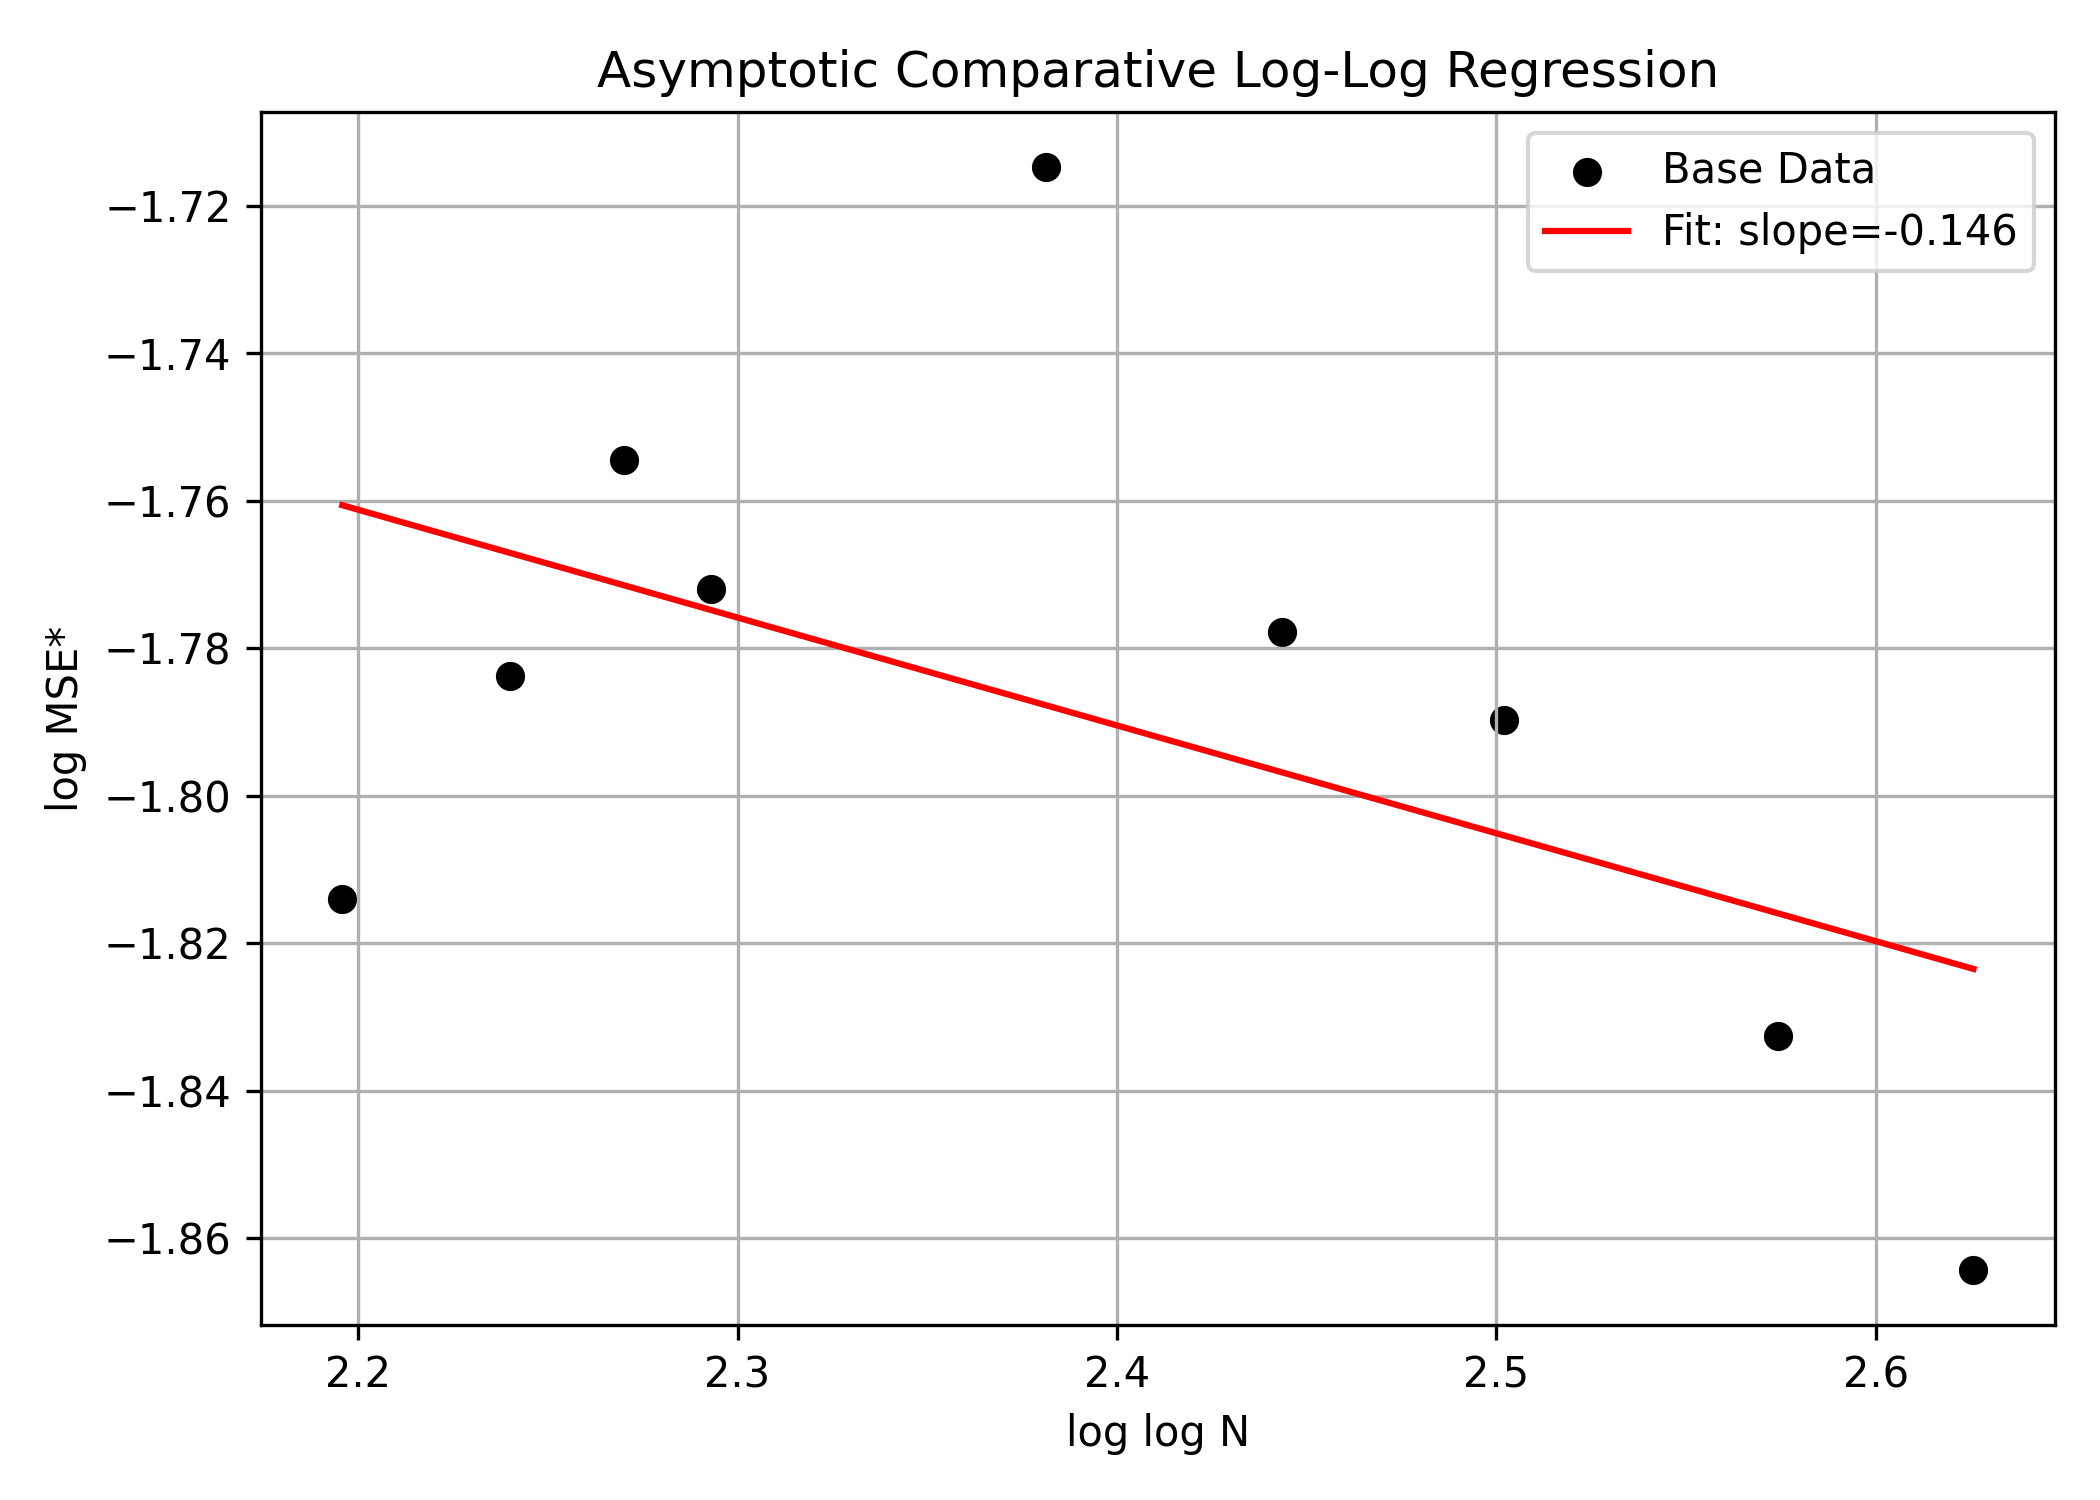
\includegraphics[width=0.8\textwidth]{figures/asymptotic_curve.png}
\caption{Comparative log-log regression between base (black/red) and boosted (blue/purple).}
\end{figure}

\appendix
\section{Appendix A}
\verbatiminput{appendixA.py}
\end{document}
